\section{Introduction} \label{sec:intro}
Education is important in developing future generations. But, even in today's society, there is large amounts of inequality in education. A study done by NPR \cite{npr2016} studies the spending of school districts throughout the United States. The article discusses the large inequality in student spending by district, noting that districts in close vicinity may have large gaps in spending. The education inequality comes partly from income inequality, since much funding for schools comes from local taxes. In lower income regions, families pay less taxes and in turn schools are more likely to be under resourced and spend less per student compared to regions with businesses and higher income families. This lower spending affects students' educational attainment \cite{spending2015, spending2017}. Figure \ref{fig:poverty} shows the poverty levels in the United states taken from the NCES MapED interactive map\footnote{\href{https://nces.ed.gov/programs/maped/map.aspx}{https://nces.ed.gov/programs/maped/map.aspx}}. From this figure we see that poverty levels have some relation to district spending when comparing to Figure \ref{fig:spending}. Following from these observations, we wish to study the link between school performance and income inequality. From this study we hope to discover key properties of well performing schools that may suggest ways to decrease this education gap. 

\begin{figure} 
	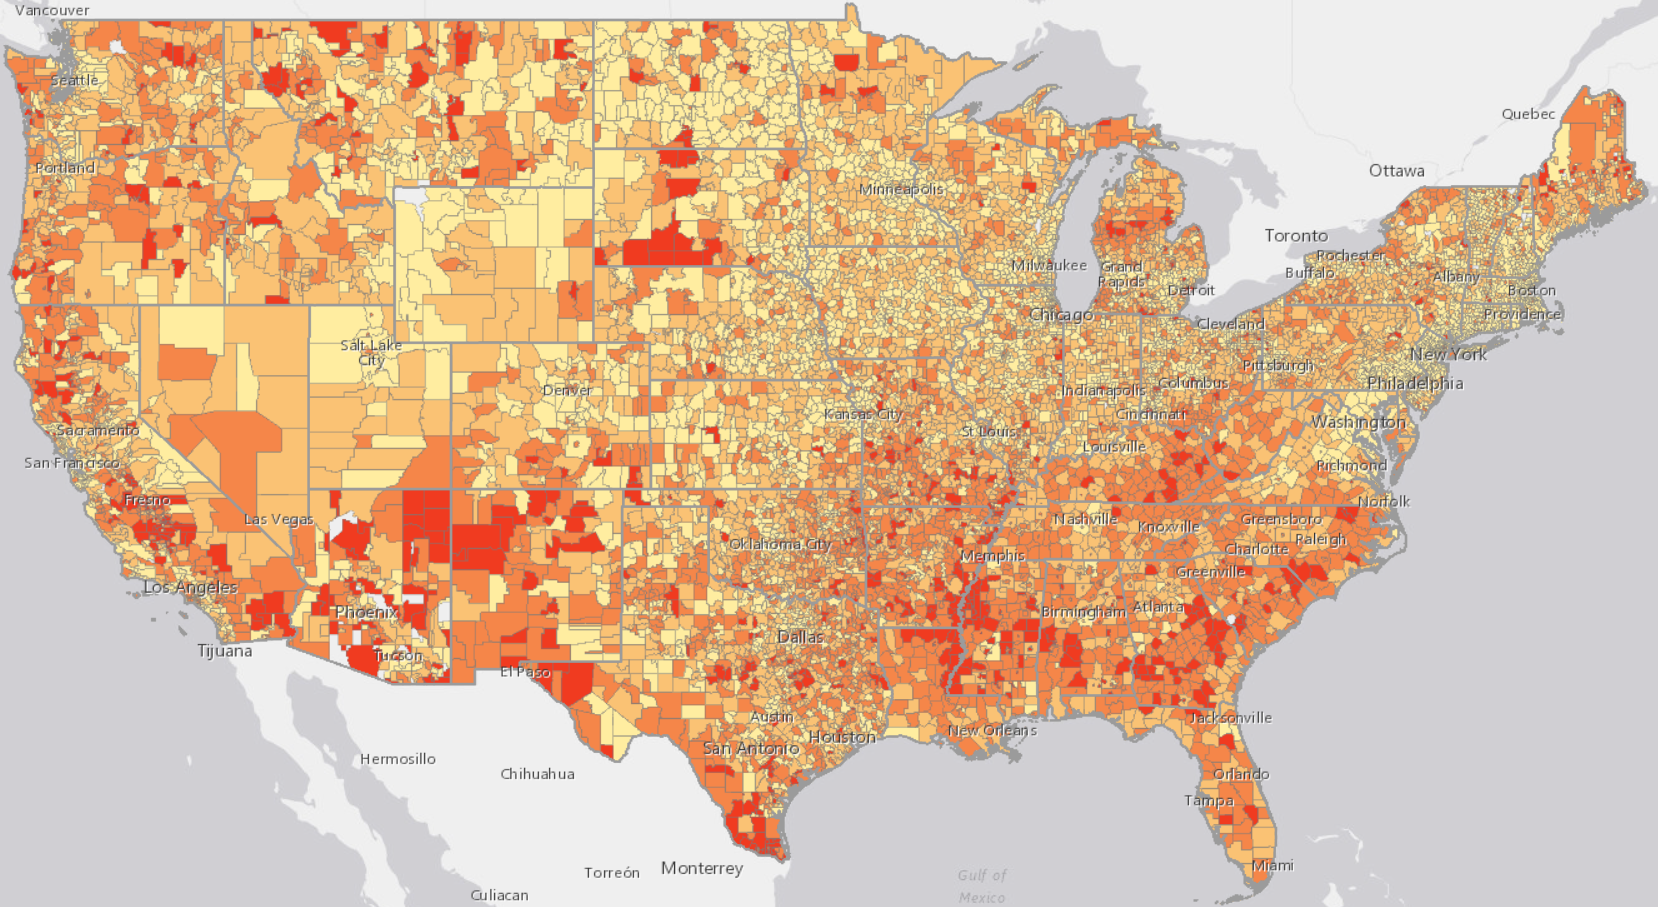
\includegraphics[width=8.45cm]{images/poverty_us.png}
	\caption{Poverty levels in the United States for those under 18 years old. Yellow colors are low poverty rates while darker, redder colors are higher poverty levels.}
	\label{fig:poverty}
\end{figure}

Our goal is to find patterns in school and census data that may suggest ways to decrease inequality in the education system. We will be looking at integrated school data from the National Center for Education Statistics (NCES) Common Core of Data (CCD) and the US Census Bureau American Community Survey (ACS) data. The former data, contain administrative data such as number of students and number of teachers. The Department of Education also has The EDFacts Initiative website that contains student proficiency by schools which will help in evaluating and comparing performance. The ACS data are information on average income level of families in each state by district. We wish to link these two datasets to discover important variables that may show ways to improve education.

We join these datasets based on individual schools to obtain properties for each school. Using student subject proficiency provided to evaluate performance, we will study the effects of variables that increase or decrease a schools performance level. In this way, we may be able to infer some important properties which can suggest ways to improve education quality in schools that perform poorly. We suggest that income level of families plays an important part, but we wish to discover other key factors that affect education, such as universe information of schools (number of students, number of teachers) and district fiscal information (local and state revenue).

For our model, we propose a homogeneous network for measuring school performance, where a node represents a school, and links between schools are based on geographic distances between schools. Node attributes will be gathered from the CCD and EDFacts dataset to get important administrative and logistics information of schools. We also will use reading and math proficiency scores to evaluate school performance. We propose to bin schools into discrete classes based on school performance. Using the ACS data, we can measure poverty of children within each school district to account for income inequality between different school areas. The proposed network should capture the similarities of schools based on their district and geographic location. Since much of school funding comes from the state and local (district) level, we believe schools close to each other (such as in the same district) will have similar performance due to similarities in spending and income levels in nearby areas. Also, due to the nature of school funding, we propose to restrict links to schools that are in the same state.

To discover important features we consider the problem of education gaps as a classification task which classifies schools into performance bin (i.e. very good, good, bad, etc.) and determine features that are important. We will compare traditional methods in machine learning such as random forest models for feature ranking and classification, and compare classification performance with network based features and algorithms. We propose that treating schools independently of location and connections does not provide good results compared to relational algorithms.

\begin{figure} 
	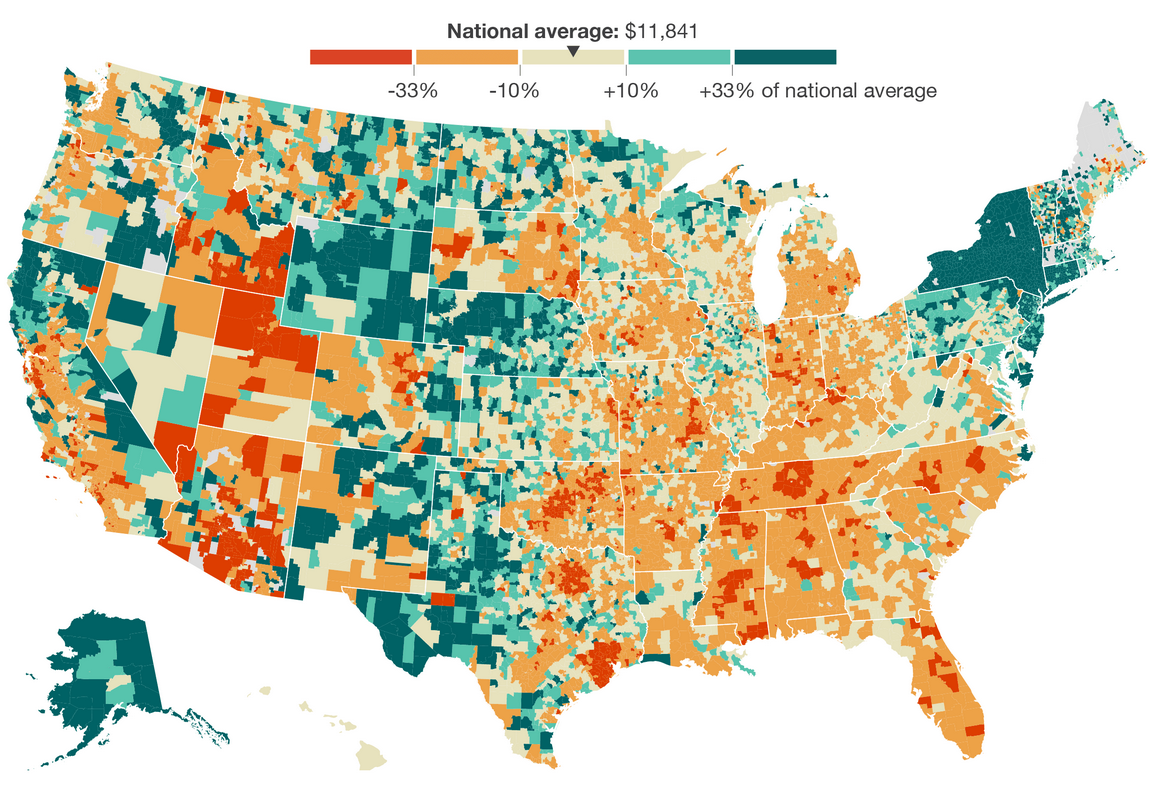
\includegraphics[width=8.45cm]{images/spending2016.png}
	\caption{Spending per student in each school district}
	\label{fig:spending}
\end{figure}

\section{Related Work} \label{sec:relwork}

Education in general is a well studied problem in the social sciences field. From the literature, child achievement can be attributed to a number of factors such as socioeconomic status or resources available at school. Studies have been done on the effect of parental education as well as family income on educational achievement on children \cite{parentinfluence2005}. Davis-Kean found that socioeconomic factors play an indirect role to a child's academic achievement, such as parents' belief and behaviors. Parents' education level was also found to be an important factor when looking at school children. Further studies done in the school performance of Australia \cite{australiaschool2004} attribute five main factors which affect school performance: previous student attainment, socioeconomic status of the students, school size\footnote{Shows that as school size falls below 1,000 students, average student attainment falls too.} (based on number of students), location type (rural or urban), and school sector (public, private, or Catholic). Furthermore, studies have show the importance of higher education attainment and equal distribution of education help to make income distribution more equal \cite{income2002greg, income2015breen}. An article published on NPR \cite{npr2016} studies the differences in education spending throughout the United States. They show that spending on education varies widely in the U.S., and look at the poor condition that some schools are in. Figure \ref{fig:spending} shows the United States spending per student for each school district. Studies have shown that spending per student have an affect on educational attainment \cite{spending2015, spending2017}, however, in \ref{sec:data} we see that this may not be the case when measuring average subject proficiency levels per school.

Feature importance and selection algorithms are important part in discovering what factors lead to good predictions. Trees are a very simple and interpretable method for feature selection. Random forest has been shown to be an effective method in ranking the importance of variables in a natural way \cite{breiman2001random}, and is a very powerful ensemble learning method. Henderson et al. \cite{recursive2011} present a feature extraction algorithm that combines local features with neighborhood features to output regional features. An unsupervised feature selection used on networked data was developed by Li et al. \cite{robustfeature2016} that is robust to noisy links. Much work has been done on classifying networked data, and algorithms have shown in cases when nodes are not independent, collective classification performs better than traditional methods \cite{collective2008}.

\section{Problem Description} \label{sec:problem}

We consider the problem of predicting school performance. Define the school network as $\mathcal{G} = (\mathcal{E},\mathcal{S}, \mathcal{A})$. Let $\mathcal{S} = \{s_i\}$ be a set of schools where each $s_i$ is a node in the graph. Each school $s_i$ has a set of attributes denoted by $a_i \in \mathcal{A}$. Denote $e_{ij} \in \mathcal{E}$ as an edge between two schools $i$ and $j$, where $\mathcal{E}$ is the set of edges. Each edge $e_{ij}$ has a weight denoted by $w(e_{ij})$.

We formulate the prediction of a school in the form of a collective classification problem \cite{collective2008} using Gibbs sampling. Let $\mathcal{S}_o$ denote the set of schools whose performance is known and $\ms_u = \ms \setminus \ms_o$ denote the set of schools whose values need to be determined. Let $\mathcal{N}$ be the neighborhood function where $\mc{N}(s_i)$ returns the set of neighbors of $s_i$. Our task is to label all $s_i' \in \ms_u$ using $\mc{N}(s_i')$. For each unobserved node $s_i'$ we train a local classifier $f_i$ using the attributes and labels of neighbors $\mc{N}(s_i')$, then use the $f_i$ to predict the performance of $s_i'$. Since $s_i'$ may have neighbors that are unobserved, we perform a bootstrapping step where $f_i$ is trained only on the observed neighbors. Then the classifier is trained, we predict the performance of $s_i'$ and give it a label. After bootstrapping we train $f_i$ on all neighbors of $s_i'$ and perform the prediction iteratively until a threshold number of iterations has occurred. Next, we perform another set of iterations and during each iteration, we calculate the feature importance for each classifier and aggregate the results to determine predictive features in classification. During the final set of iterations, we keep track of the number of times $s_i'$ was assigned each label (-1 or 1) and give a final label assignment based on which label was assigned the most.

In summary the problem is given as follows:\\

\noindent\hangindent=.5cm\textbf{Given} a graph $\mathcal{G} = (\mathcal{E},\mathcal{S}, \mathcal{A})$ with node attributes, a neighborhood function $\mc{N}$, and with an edge weight function $w$;

\noindent\hangindent=.5cm\textbf{Train} classifiers to classify $s_i \in \ms_u$ using the features of $s_i$ using the edges and weights defined; 

\noindent\hangindent=.5cm\textbf{Predict} the performance level of all schools $s_i \in \ms_u$ using the individual classifiers;

\noindent\hangindent=.5cm\textbf{Identify} predictive features for predicting performance level of schools.

\begin{table}
	\resizebox{8.45cm}{!}{
		\begin{tabular}{p{3.75cm}p{4.95cm}}
			\toprule
			Number of Students Reported & Ranges used for Percent Proficient\\
			\midrule
			<6 & 'PS' \\
			\midrule
			6-15 & <50\%, $\geq$50\% \\
			\midrule
			16-30 & $\leq$20\%, 21-39\%, 40-59\%, 60-79\%, $\geq$80\% \\
			\midrule
			31-60 & $\leq$10\%, 11-19\%, 20-29\%, 30-39\%, 40-49\%, 50-59\%, 60-69\%, 70-79\%, 80-89\%, $\geq$90\% \\
			\midrule
			61-300 & $\leq$5\%, 6-9\%, 10-14\%, 15-19\%, 20-24\%, 24-29\%, 30-34\%, 35-39\%, 40-44\%, 45-49\%, 50-54\%, 60-64\%, 65-69\%, 70-74\%, 75-79\%, 80-84\%, 85-89\%, 90-94\%, $\geq$95\%\\
			\midrule
			More than 300 & $\leq$1\%, 2\%, \dots, 98\%, $\geq$99\% \\
			\bottomrule
			\\
		\end{tabular}
	}
	\caption{Ranges used for reporting percentages.}
	\label{tab:ranges}
\end{table}

\section{Proposed Method} \label{sec:propose}

Since the responsibility for a majority of education funding is on the state level, we propose to restrict edges in the school network for schools in the same state. Formally:

%\begin{displaymath}
%w(e_{ij}) = 
%	\begin{cases}
%	d_{ij}  & : a_{i}.state = a_{j}.state\\
%	0  & : o.w.
%	\end{cases}
%\end{displaymath}

%\begin{displaymath}
%	\begin{cases}
%	e_{ij} \in \mc{E}  & \text{if } a_{i}.state = a_{j}.state\\
%	e_{ij} \notin \mc{E}  &  o.w.
%	\end{cases}
%\end{displaymath}

\begin{displaymath}
	\mc{E} = \left\{ e_{ij} : a_i.state = a_j.state \right\}
\end{displaymath}

\noindent where $a_i.state, a_j.state$ are the states where schools $i,j$ are located, respectively. The weight of edge $w(e_{ij})$ is defined as the multiplicative inverse of the distance between schools $i$ and $j$, $d_{ij}$ , in miles as calculated by the Haversine distance formula:

\begin{equation*}
a = sin^2\left(\frac{\varphi_j-\varphi_i}{2}\right) + cos(\varphi_i) \cdot cos(\varphi_j) \cdot sin^2\left(\frac{\lambda_2 - \lambda_1}{2}\right),
\end{equation*}
\begin{equation*}
c = 2 \cdot atan2( \sqrt{a}, \sqrt{1-a})
\end{equation*}
\begin{equation*}
w(e_{ij}) = d_{ij} = R \cdot c,
\end{equation*}

\noindent where $\varphi_i, \varphi_j$ are the latitude values, $\lambda_i, \lambda_j$ are the longitude values of $s_i, s_j$ in radians, respectively, $R$ is the approximate radius of the Earth in miles, and $atan2$ is the multi-valued inverse tangent. This weight is normalized to be between 0 and 1 per school. That is, given a pair of schools in New York, $s_i, s_j$ and a pair of schools in Delaware, $s_m, s_n$, that have the same distance say 50 miles, it is possible $w(e_{ij}) \neq w(e_{mn})$. 

Given the defined structure we observe that the network has multiple densely connected communities that are defined by state. In order to capture the effect of regional differences in each state, we further propose to restrict the links. Let $
\rho$ be defined as the percentage of neighbors to keep for any node and define $|{\mc{N}(s_i)}| = n$. For a school $s_i$, define $\mc{N}_d(s_i)$ to be the neighborhood of $s_i$ sorted in descending order by edge weight. Then define $\mc{N}'(s_i)$ as the neighborhood graph such that $|\mc{N}'(s_i)| = \ceil{\rho n}$, and $\mc{N}'(s_i)$ is defined as:

\begin{displaymath}
\mc{N}'(s_i) = \left\{ s_j \in \mc{N}_d(s_i) : s_j.index \leq \ceil{\rho n} \right\}
\end{displaymath}

So $N_i'$ is the neighborhood of school $s_i$ with only the closest $\rho\%$ number of schools in the state as its neighbors. We propose that similar schools in the same state and similar region have a greater effect on the prediction of performance for a school. For each unobserved node $s_j$, a local classifier is trained based on the observed neighbors in $N_j'$ in the manner discussed in Section \ref{sec:problem}. For each local classifier, samples are weighted by their edge weight $w$.

\begin{figure}
	\begin{subfigure}{.2325\textwidth}
		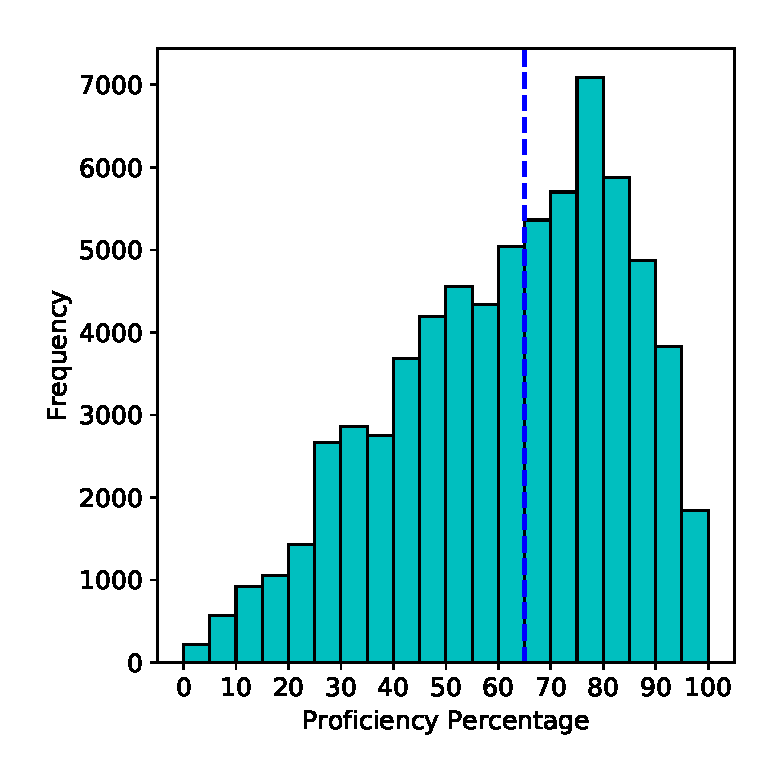
\includegraphics[width=\linewidth]{images/prof_math}
		\caption{Math proficiency}
	\end{subfigure}
	\hspace{\fill}  % for some horizontal separation 
	\begin{subfigure}{.2325\textwidth}
		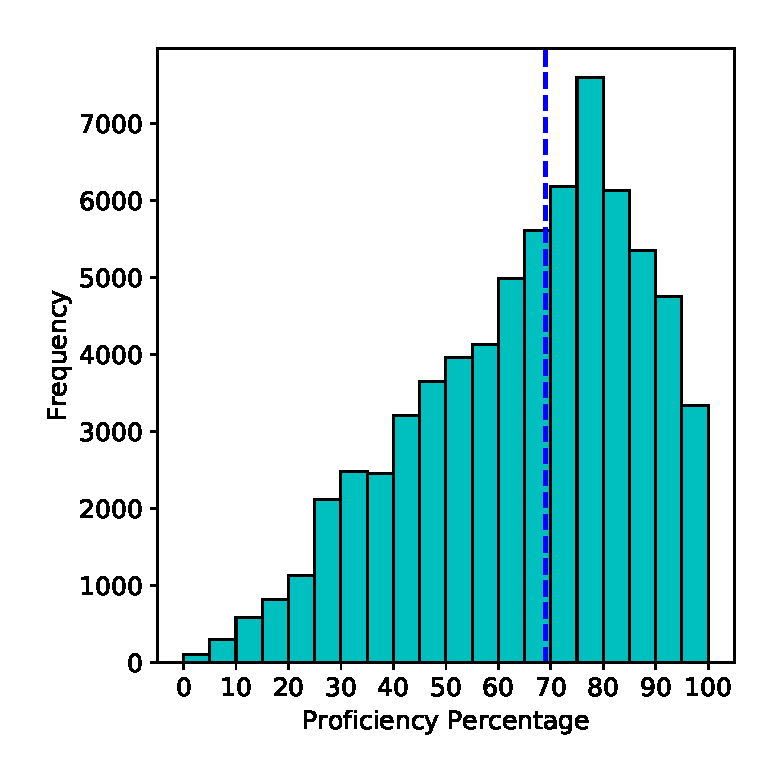
\includegraphics[width=\linewidth]{images/prof_read}
		\caption{Reading proficiency}
	\end{subfigure}
	\caption{Distribution of proficiency levels for both math and reading/language arts. Dashed line shows the median proficiency level.}
	\label{fig:prof}
\end{figure}

\section{Dataset Description} \label{sec:data}

We explore school level data and census data to quantify and measure factors that affect educational attainment. For now we focus on the 2013-2014 school year, but we hope to have a framework for implementing data from multiple reporting years.

\subsection{Data Collection} \label{sec:collect}

Our dataset comes from multiple government resources which we will discuss in detail. School level information and statistics is provided by the NCES CCD\footnote{\href{https://nces.ed.gov/ccd/pubschuniv.asp}{https://nces.ed.gov/ccd/pubschuniv.asp}}. The data is provided as a means to provide consistent, reliable data to U.S. Department of Education and researchers in addressing education needs \cite{ccdschool}. The public school universe data covers the 50 states, the District of Columbia, and five U.S. Island Areas (American Samoa, Guam, the Commonwealth of the Northern Mariana Islands, Puerto Rico, and the U.S. Virgin Islands). This dataset contains school logistics information such as number of students, number of full-time equivalent teachers, and information on school programs (e.g. status of the National School Lunch Program or Title I status). The CCD website also has datasets of district level fiscal information, which we will also use as features for school level prediction. District fiscal information includes variables on spending and revenue at the local and state level.

To add more information to get better overall view on school performance we use the ACS\footnote{\href{https://www.census.gov/programs-surveys/acs/}{https://www.census.gov/programs-surveys/acs/}.}
data by the U.S. Census Bureau, which provides district area  poverty levels. Family income plays an important part in educational attainment \cite{parentinfluence2005} so we link the CCD and ACS data to provide information on poverty levels per school district. We believe this will be a strong predictor in the prediction task.

To assess the performance of schools we use data collected by the U.S. Department of Education EDFacts initiative \footnote{\href{https://www2.ed.gov/about/inits/ed/edfacts/data-files/index.html}{https://www2.ed.gov/about/inits/ed/edfacts/data-files/index.html}}, and use reading/language arts and mathematics achievement to evaluate school performance. The data measures the percentage of students that scored at or above proficient in the given subject. To protect privacy of students, the Department has blurred data based on a tier for number of students per school. Table \ref{tab:ranges} shows the ranges used percentage of proficient students for the number of students per school. Schools with less than 6 students were suppressed with 'PS'.

\begin{figure} 
	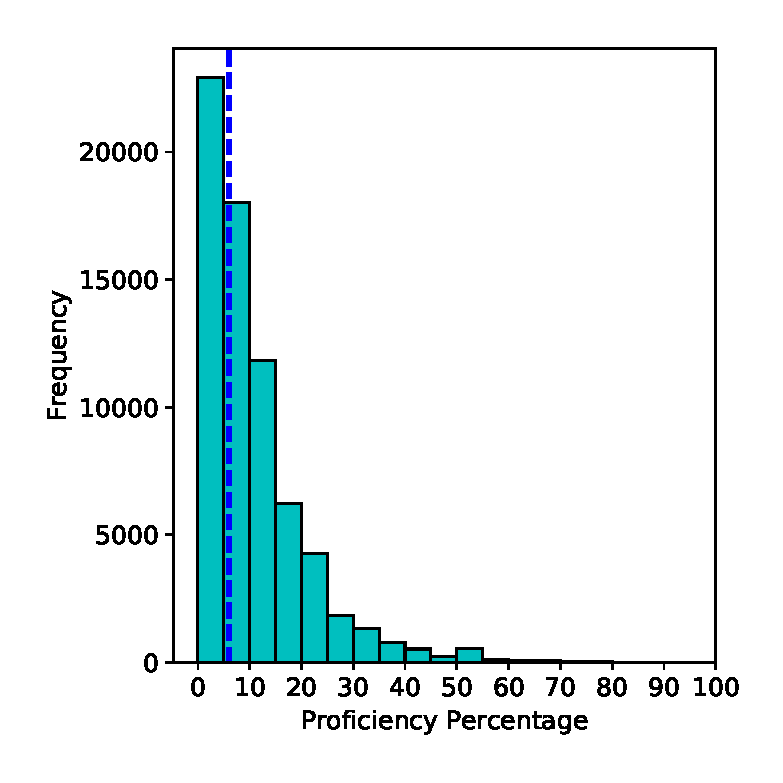
\includegraphics[width=7.5cm]{images/prof_diff}
	\caption{Distribution for the difference of math and reading proficiency level. Dashed line shows the median difference between subject proficiency level.}
	\label{fig:diff}
\end{figure}

%\begin{figure}
%	\begin{subfigure}{.2325\textwidth}
%		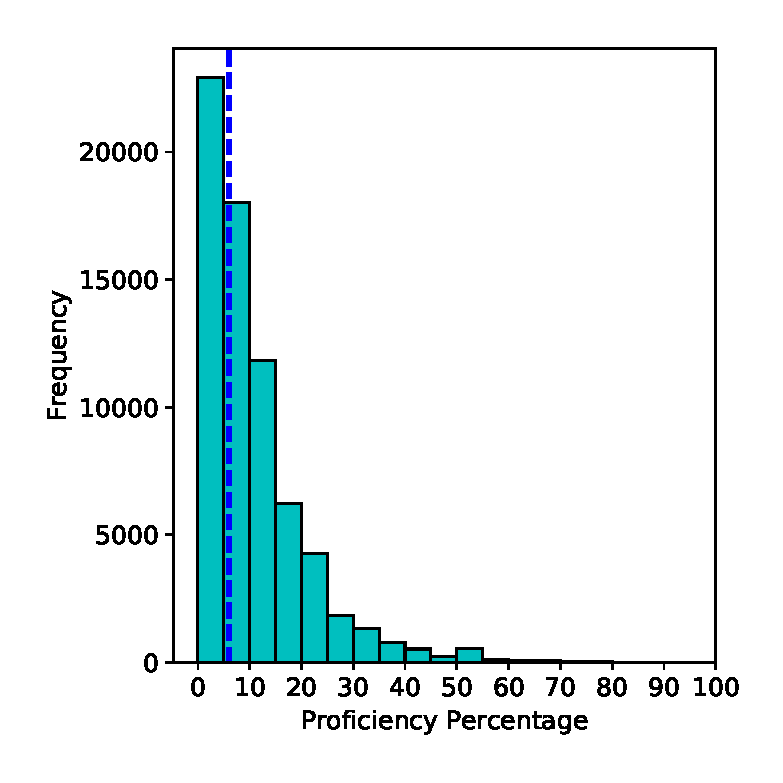
\includegraphics[width=\linewidth]{images/prof_diff}
%		\caption{Distribution for the difference of math and reading proficiency level. Dashed line shows the median difference between subject proficiency level.}
%	\end{subfigure}
%	\hspace{\fill}  % for some horizontal separation 
%	\begin{subfigure}{.2325\textwidth}
%		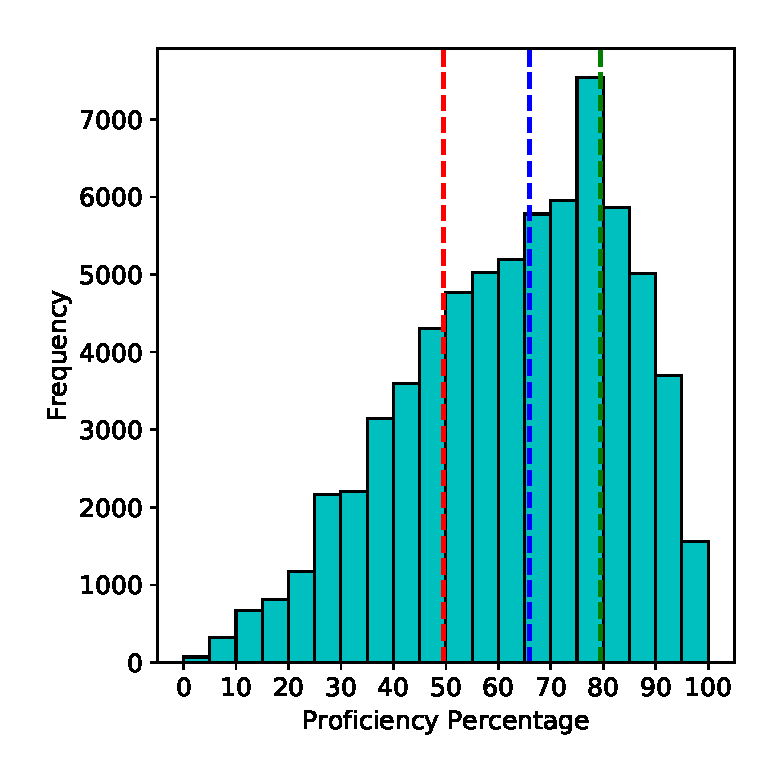
\includegraphics[width=\linewidth]{images/prof_avg}
%		\caption{Distribution for the average between math and reading proficiency levels. Red dashed line is $Q_1$, blue dashed line is the median, and green dashed line is $Q_3$.}
%	\end{subfigure}
%	\caption{Distribution of proficiency levels for both math and reading/language arts. Dashed line shows the median proficiency level.}
%	\label{fig:profavg}
%\end{figure}

The datasets discussed previously are self-reported by states and school districts. Naturally this will lead to unreported information or missing values in the school universe and district fiscal information. To deal with this issue, we drop entries with missing values. In the case of the school proficiency dataset, entries with a suppressed value are removed, along with schools with less than 16 students to avoid the large ranges in proficiency created by using a schools with low number of students. In addition, the school universe dataset has categorical columns in which a valid value is "N" for "not applicable." We treat these values as a separate category when training our classifiers. Furthermore, the district fiscal information has entries that have a value of 0 in the total revenue column and -1 for missing data. Since we consider district spending an important feature \cite{spending2015,spending2017} we drop entries that do not report, or are missing revenue information. Finally, there are numerous extraneous variables in the data file, so we remove these extraneous information for our prediction task. Extraneous variables include things like phone number, four digit zip code, and other unimportant identifying factors of schools.

\begin{figure} 
	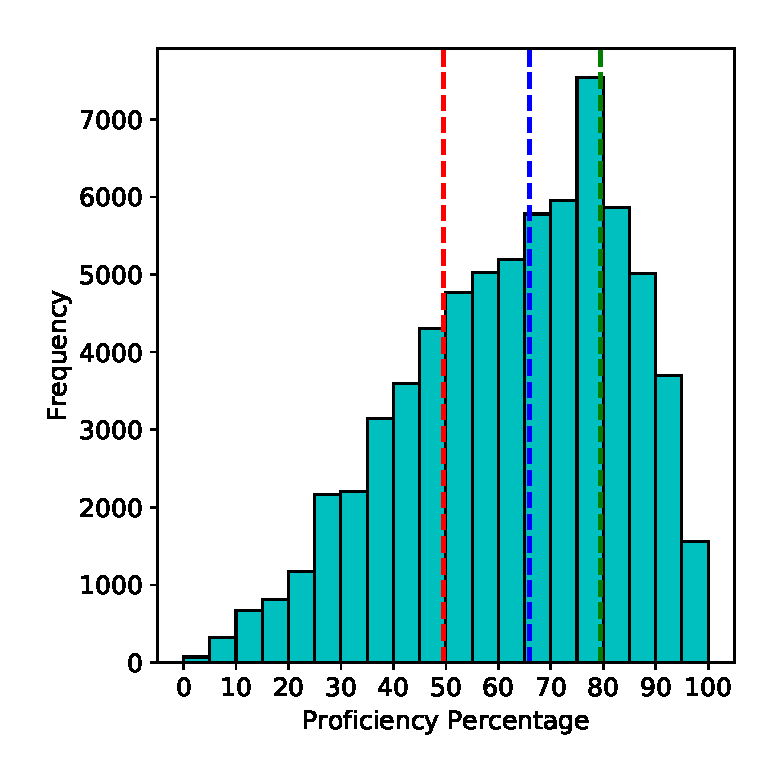
\includegraphics[width=7.5cm]{images/prof_avg}
	\caption{Distribution for the average between math and reading proficiency levels. Red dashed line is $Q_1$, blue dashed line is the median, and green dashed line is $Q_3$.}
	\label{fig:avgprof}
\end{figure}

\subsection{Data Processing} \label{sec:processing}

We wish to use the datasets described in \ref{sec:collect} to identify key factors that contribute to school performance. Since the datasets are from separate sources, we take advantage of unique school IDs and district IDs to join the school universe information, district fiscal, poverty level, and math and reading proficiency datasets. After cleaning and joining the data the final number of observations were 68,850.

To quantify school performance, we combine the reading/language arts proficiency file with the mathematics proficiency file, and "bin" schools based on percentage of proficient students. The school proficiency was calculated by taking the average of the reading/language and mathematics proficiency. We then wish to label each school based on the percentage proficiency. To transform our task of predicting school performance into a binary classification problem, we need to bin schools into two classes: "good" and "bad". Figure \ref{fig:prof} shows the distribution of proficiency levels for math and reading subjects. We can observe that the distributions for each of the subjects are skewed to the right. Before binning the schools based on performance on math and reading, we first plot a distribution of the absolute difference in proficiencies of math and reading. Figure \ref{fig:diff} shows the distribution of absolute difference in percentage proficiency for math and reading. We observe that in most cases, there is very little difference between the percentage of proficient students in math and the percentage of proficient students in reading, however, there are outliers where the difference is very large. For example there is a school with about 95\% of students who were proficient in math but only about 5\% students who were proficient in reading.

To deal with the problem of outliers in the differences of proficiency levels, we take the average between math and reading. After calculating the average, we will use a boxplot method to divide the dataset and remove the outliers mentioned previously. The average score distribution is shown in Figure \ref{fig:avgprof}. We observe that this distribution is also slightly skewed to the right since the math and reading scores were both skewed to the right. Using the same idea of constructing a boxplot, we calculate the median, first quartile ($Q_1$), and third quartile ($Q_3$) values. We take all schools with proficiency levels greater than or equal the $Q_3$ as well performing schools (labeled as class 1), levels less than the $Q_1$ as poor performing schools (labeled as class -1), and leave schools with levels in between as neutral (labeled as class 0). In this way we have a more clear idea of what schools are well-performing vs poor-performing and remove schools whose differences in subject proficiency is too high.

\section{Experiments} \label{sec:experiment}

Our experiments are done on the final, cleaned, and processed 2013-2014 school year data discussed in Section \ref{sec:processing}. First we do some data analysis and compare school performance and look at the distribution throughout the United States. Then we perform our classification experiments and compare traditional machine learning method to the relational methods.

\begin{table}
	\resizebox{7cm}{!}{
	\begin{tabular}{ccc}
		\toprule
		Class & Number of Observations & Percentage\\
		\midrule
		-1 & 18398 & 26.72\% \\
		\midrule
		0 & 32555 & 47.29\% \\
		\midrule
		1 & 17897 & 25.99\% \\
		\bottomrule
		\\
	\end{tabular}
	}
	\caption{Statistics about the education dataset.}
	\label{tab:classes}
\end{table}

\subsection{Analysis} \label{sec:analysis}

Figure \ref{fig:us} shows the United States map with schools colored by performance bin. Green represents schools that have good performance, yellow are schools that have a neural performance, and red signify schools with poor performance, based on our labeling method discussed in Section \ref{sec:processing}. Note that not all schools in the United States are shown on the map, most notably in Kansas, South Dakota, and Minnesota. As discussed in Section \ref{sec:collect}, there were many missing values that were due to data collection errors or unreported values. These observations that contained missing values were dropped, which explains the large gap in missing schools. There are probably various reasons that the schools in the east side have less issues in the data set than the west side, but we do not explore these issues in this paper.

One observation that we can make from Figure \ref{fig:us} is that often school performance varies widely by state, but does not vary much within states. That is, states usually have a majority of poor performing or well performing schools. This is most notable in the south Great Lakes region such as Indiana and Ohio which have a majority of well performing schools, or in the mid-southeast region in Tennessee or South Carolina that have a majority of poor performing schools. This suggests that state policy regarding education probably has an affect on educational achievement, but this is probably not verifiable within the data, since this requires analysis of political policies between states. However, it may be possible that different district fiscal information such as revenue due to local and state taxes can capture part of these differences.

\begin{figure} 
	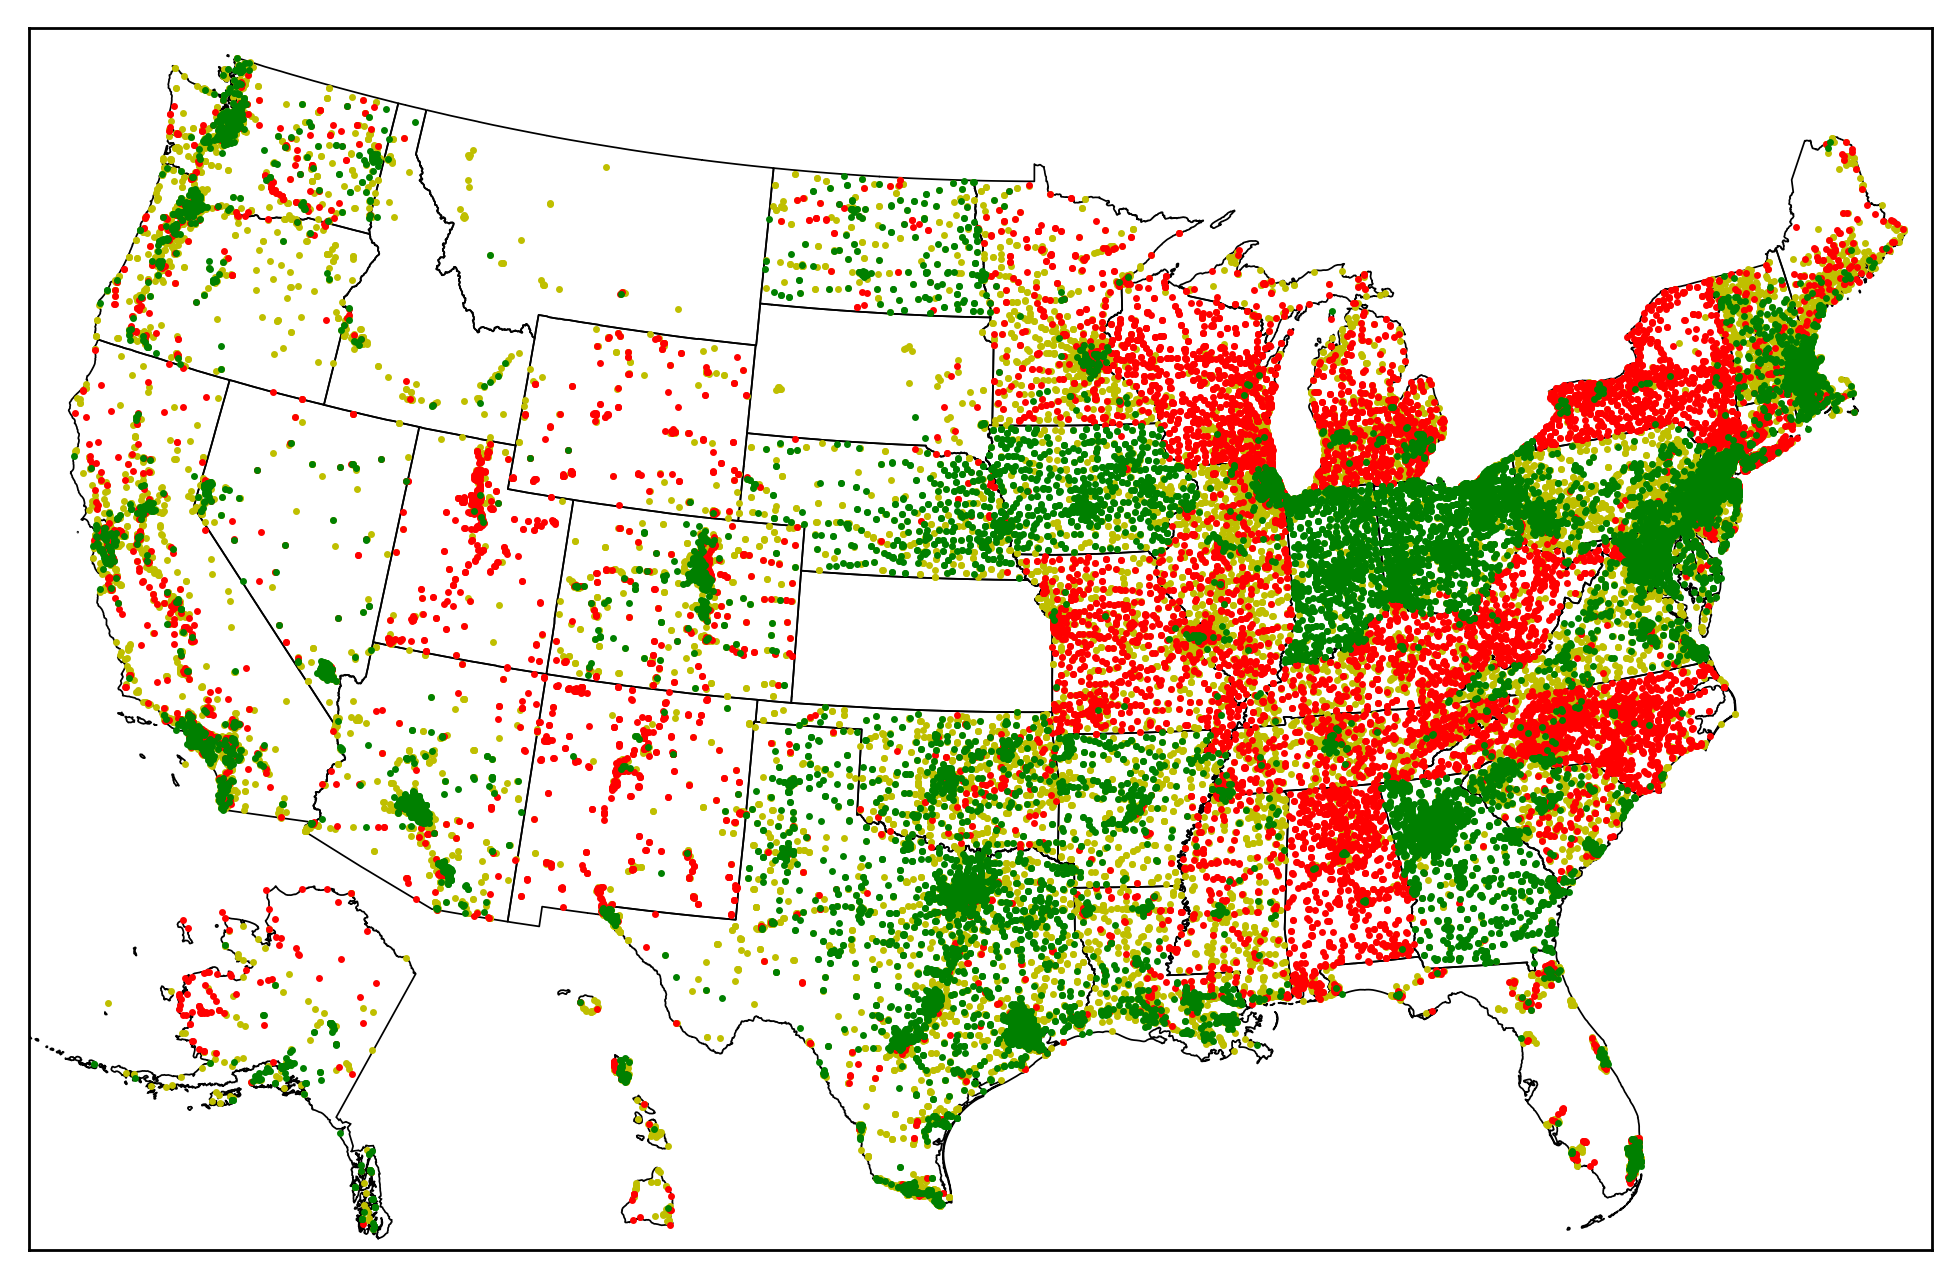
\includegraphics[width=8.45cm]{images/avg_us.png}
	\caption{Map of the United States with schools plotted. Green dots are schools that have good performance, yellow dots are schools that have a neutral performance, and red dots are schools that have poor performance.}
	\label{fig:us}
\end{figure}

In addition, we can compare the results on our east United States map to the map in the NPR article \cite{npr2016} in Figure \ref{fig:spending}. Although our dataset is from the 2013-2014 school year and the NPR study was done in 2016, we still believe there can be some comparisons done to the distribution of scores throughout the United States compared to the spending per student. Since our west side is missing many schools we do some comparisons by state in the east coast. One important observation we can make is that New York overwhelmingly spends more per student than the national average, but school proficiency is mostly poor throughout the state. If we take a close look at the regions that have well performing schools in New York, they are generally high population areas such as clusters of green in Buffalo, Rochester, and New York City. This can be further observed in a state such as Michigan, where most well performing schools are located near Detroit, Lansing, and Grand Rapids. Comparing these results to Figure \ref{fig:spending}, we see that the spending per student does not necessarily correlate to school performance. Other than New York, another region that shows this difference is the Indiana and Ohio region, since those states often spend less than the national average, but have better proficiency than other states.

Furthermore, comparing our map of test scores to Figure \ref{fig:poverty}, we can see that there is some relation to poverty levels to school performance. Again taking the examples of Indiana and Ohio, we see that the poverty levels are relatively low in that region, while good school performance is overwhelmingly the majority. This matches our original thoughts on the effect of income on education performance.

\subsection{Evaluation} \label{sec:evaluation}

\begin{figure*}
	\begin{subfigure}{.45\textwidth}
		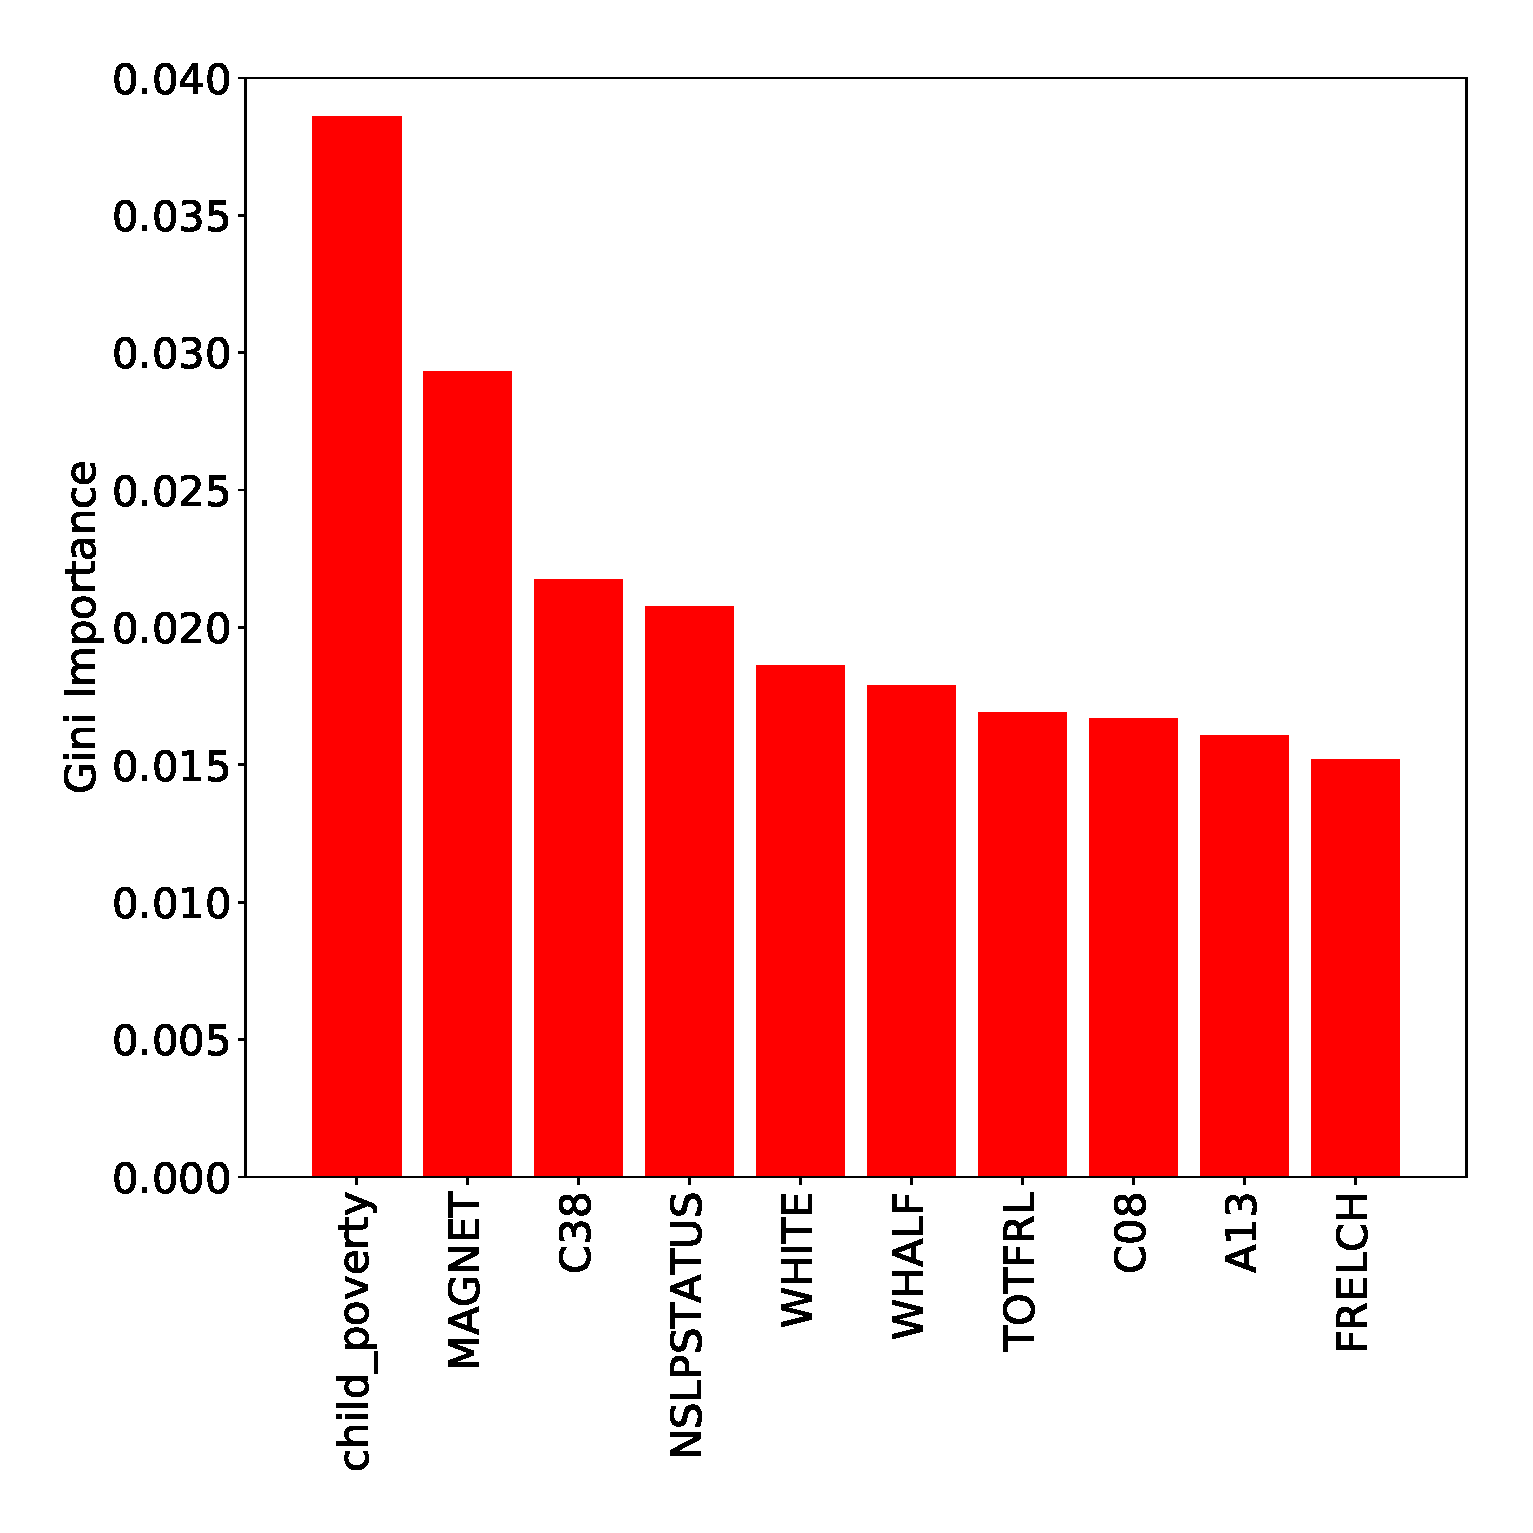
\includegraphics[width=\linewidth]{images/features_rf}
		\caption{Random Forest}
	\end{subfigure}
	\hspace{\fill}
	\begin{subfigure}{.45\textwidth}
		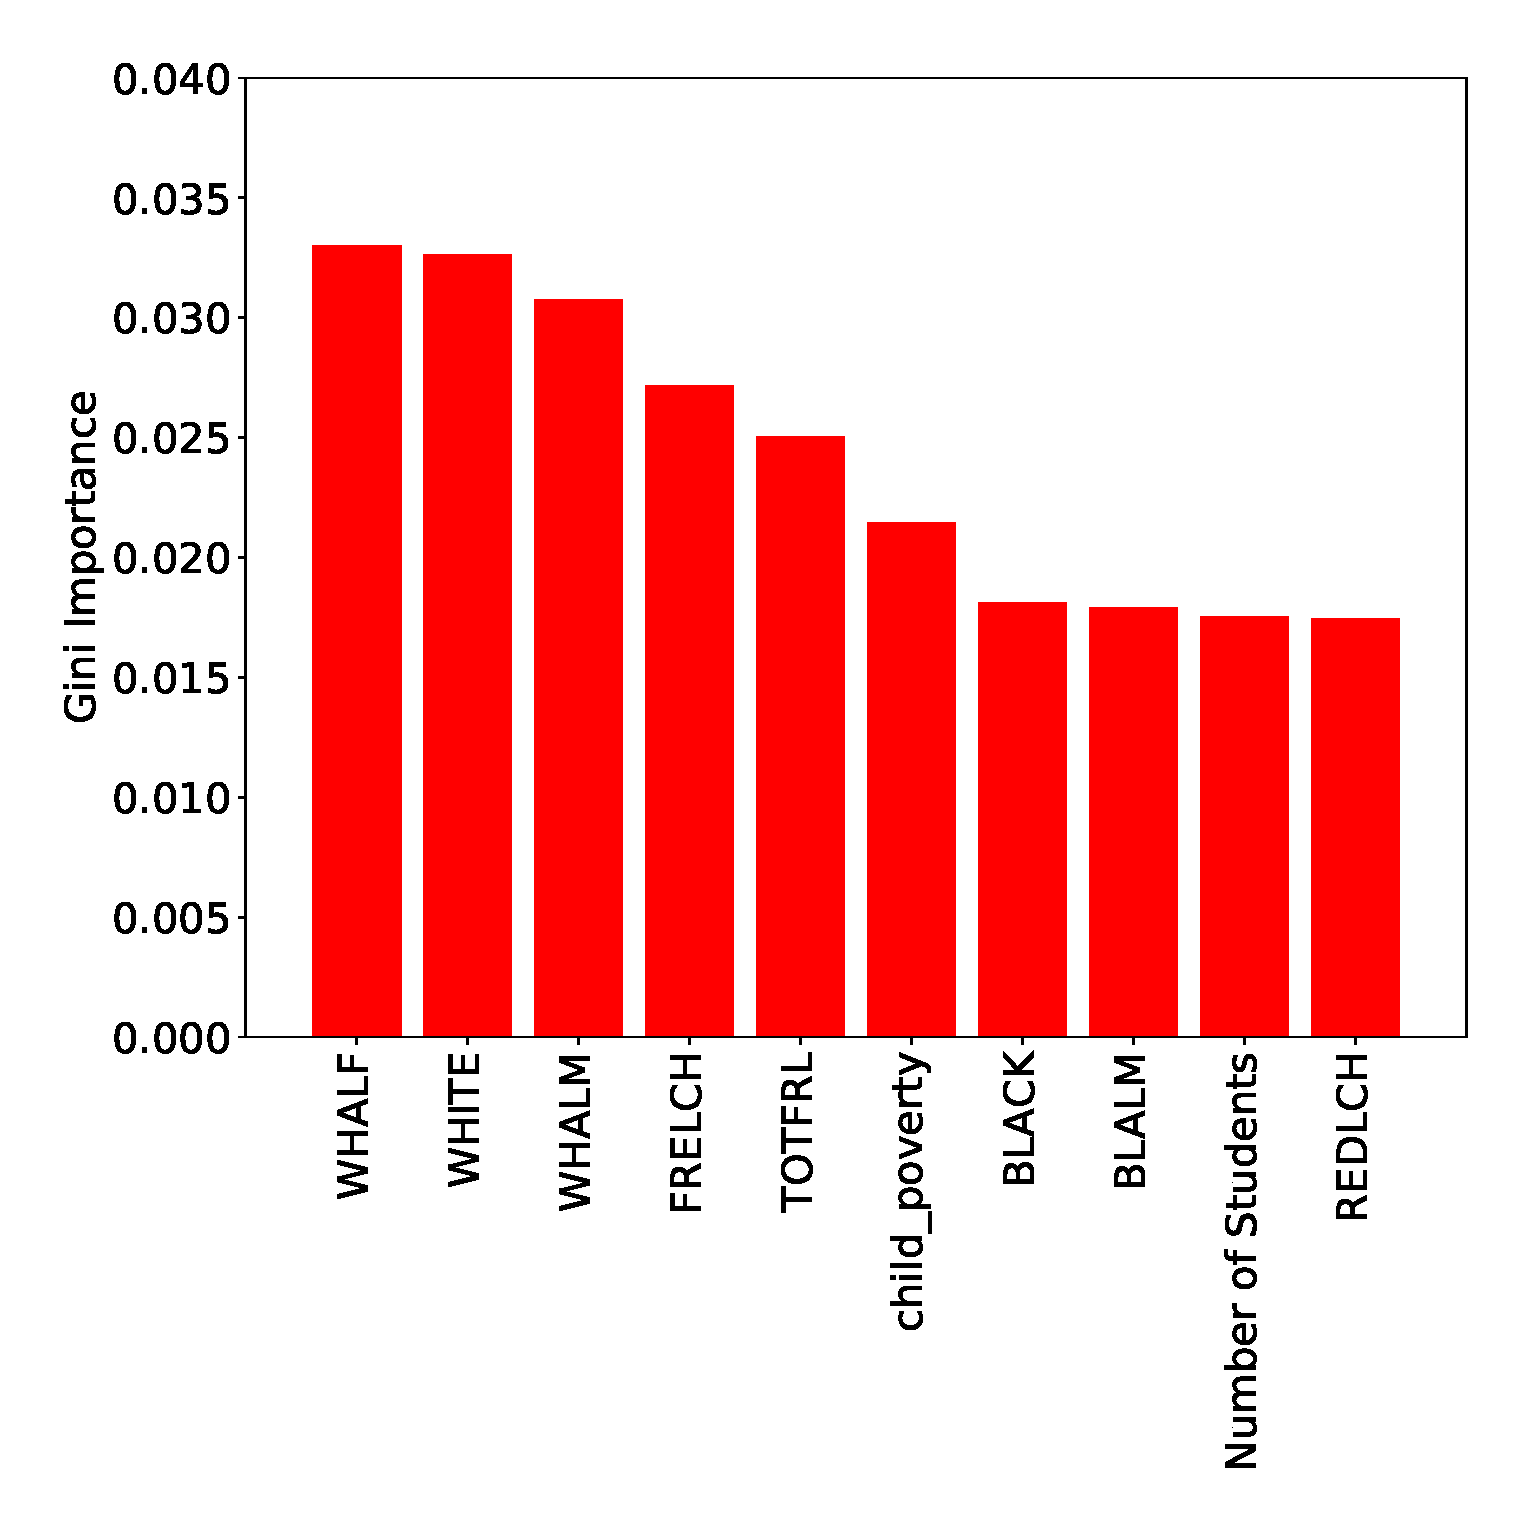
\includegraphics[width=\linewidth]{images/features_gs}
		\caption{Gibbs Sampling (RF)}
	\end{subfigure}
	\caption{Top 10 features based on gini importance for Random Forest and Gibbs sampling (RF) model.}
	\label{fig:features}
\end{figure*}

We perform a binary classification task on our dataset to predict school performance. Using the labels that we discussed in Section \ref{sec:processing}, we perform binary classification on positive and negative classes. The statistics on the class distribution is shown in Table \ref{tab:classes}. The classes are relatively balance due to the way to split the samples into the different classes. In our experiments we have a total of 36,295 observations. To evaluate our models, we split the dataset into train and test using an 80-20 split. For our baseline method, we use a traditional machine learning algorithm, a Random Forest classifier with 50 estimators, implemented using scikit-learn \cite{scikit-learn}. In this scenario, schools are treated independently of location and the whole training set is used to classify each test instance. For our proposed solution, we set $\rho = .2$ so that we keep the closest 20\% schools in the neighborhood, $N(s_i)$, of each school $s_i$. Our idea is to limit the effect on prediction for schools that are far away, which can be slightly supported by the observations made in Section \ref{sec:analysis}, where location of the school seems to matter within the state. For each unobserved node $s_i' \in S_u$ we perform the Gibbs sampling method as discussed in Section \ref{sec:problem} using a Random Forest classifier with 50 estimators. The burn in stage runs for 10 iterations and the iterative classification step runs for 50 iterations. We evaluate the models using accuracy and f-1 score. The results are shown in Table \ref{tab:results}.

Using the classifiers discussed, we wish to see which features in our dataset contribute more to prediction. To do this, we measure the importance of a feature by using the "gini importance" described in \cite{breiman1984classification}. This is defined as the total decrease in node impurity for each feature weighted by the probability of reaching the node averaged over all trees in the ensemble, normalized to be between 0 and 1. For the Gibbs sampling model, we average the gini importance of each feature over all iterations in the classification step. Figure \ref{fig:features} shows the plot of the top 10 features with their gini importance. We detail these results in Table \ref{tab:features}.

Table \ref{tab:features} give a description of some of the top features based on the gini importance. We take note that the the most important feature based on this criteria is the level of child poverty in the school district. This in part aligns with our assumption and the studies done in \cite{income2002greg,income2015breen}, which say that family income plays a role in educational attainment. Also we can see some school administrative information also plays a role in the performance of schools, such as if the school is a magnet school or not, and their participation in the National School Lunch Program. In addition, C38 and C08 are state revenue information for districts, which show where that revenue source plays some part in the performance of schools within a district. Also, we observe that our model has different feature importances than the Random Forest model. One likely reason is that each local classifier may have different feature importances, and this probably changes based on state since the distribution of schools is different per state. Since we just take the average gini importance over all local classifiers, this may affect the results.

\section{Discussion} \label{sec:discuss}

From Figures \ref{fig:poverty} and \ref{fig:spending}, we see the inequality in district spending, and that poverty levels vary widely throughout the united states. Comparing our map of test scores, we can see that there is some relation to the poverty level and performance of schools, most notably in Indiana and Ohio, where the majority of schools perform well and have relatively low poverty levels. This is further enhanced by the children poverty rate being a feature with a top gini importance ranking. From our results on feature ranking, we also see that some fiscal information for districts, as well as school federal programs such as NSLP are predictive of school performance. In our proposed model, we see that the number of students is predictive in proficiency levels. This support some findings done in the Australia school study by Lamb et al. \cite{australiaschool2004}, where one of the identified five factors that affect school performance was the size of the school. This result could potentially be generalized too United States schools as well. Additionally, it seems that demographics also play a role in predicting school performance. This may be in part due to different demographics living in different conditions, which may correlate with the poverty level in various districts, however, we do not analyze these conditions in this work. Furthermore, our gini importance values are very low. This may be because our feature space is too large for our task, so each feature has less importance overall. Another possible reason could be that all features are important relative to the feature space, and are required for predicting school performance. A possible next step would be to perform experiments using the top-\textit{k} features, and see how it affects performance of the classifiers. Finally, we should measure feature importance on a local classifier level instead of averaging over all local classifiers, to get a better view on feature importance regionally.

\begin{table}
	\resizebox{7cm}{!}{
		\begin{tabular}{ccc}
			\toprule
			Model & Accuracy & F-1 Score\\
			\midrule
			Random Forest & 0.9702 & 0.9695 \\
			Gibbs sampling (RF) & 0.9653 & 0.9648 \\
			\bottomrule
			\\
		\end{tabular}
	}
	\caption{Results on binary classification task using Random forest with 50 estimators and Gibbs sampling using Random Forest (RF) as the local classifier.}
	\label{tab:results}
\end{table}

From our classification results, we see that the traditional machine learning model is more than sufficient to predict school performance and even performs better than the collective classification model. One possible reason could be attributed to the value of $\rho$ that was selected, as this was not tuned precisely to give better results. It is possible that including less or more nodes in the neighborhood of a school could affect prediction results. Although our model did not perform better than a traditional Random Forest model, we see that classification methods can perform very well on determining whether a school is performing well or poorly. However, one caveat is that the selected schools were on the upper or lower end of the distribution for proficiency level. From these results it is not clear what would happen for schools that are in the "middle". A potential next step would be to incorporate more schools in the final dataset to see the effect on adding schools with closer levels of proficiency, and see if a classification task can be performed in this scenario. One hypothesis is that a relational method would perform better in this instance, since adding more schools blurs the lines between differences of well and poor performing schools. In our proposed relational classification method, schools would only be classified based on local performance, rather than globally such as in a traditional method.

One direction that we did not incorporate into our work is applying traditional and network based feature selection algorithms. As we previously discussed, gini importances of our features were pretty low, so it may be beneficial to select a subset of features for classification, and study the affect it has on the models. In this way we can better generalize this prediction task. Finally, we would like to study and combine multiple reporting school years in order to analyze changes in performance by year per school.

\begin{table}
	\resizebox{8.45cm}{!}{
		\begin{tabular}{p{3cm}p{5.70cm}}
			\toprule
			Feature Name & Description\\
			\midrule
			child\_poverty & The rate of child poverty. This value is measured on a district level, so all schools in a district have the same poverty level. \\ \\
			MAGNET & A binary feature on whether a school is a magnet school or not. 
			\\ \\
			NSLPSTATUS & The National School Lunch Program (NLSP) status of the school.
			\\ \\
			TOTFRL \& FRELCH & Number of Free and Reduced Lunch students.
			\\ \\
			C38 \& C08 & Features dealing with State Revenue.
			\\ \\
			WHITE \& WHALF & Number of total White, non-Hispanic students and number of total White, female students.
			\\ \\
			BLACK \& BLACKM & Number of total Black students, and number of total Black, male students.
			\\\bottomrule
			\\
		\end{tabular}
	}
	\caption{Description of some of the top features with the highest gini importance.}
	\label{tab:features}
\end{table}

\section{Conclusion} \label{sec:conclusion}

In this work we have done an analysis on school performance in the United States. Our goal was to determine if school performance can be predicted using machine learning and to find key features that are predictive of school performance. From our results, we see that in a dataset with clear division of school performance, we are able to predict proficiency levels with high accuracy. We also verify that poverty levels are important in school performance levels, as well as some school logistics and administrative information. In our work, we took a subset of the data from the top and bottom performing schools. For future steps, we would like to incorporate a larger percentage of the dataset to see the effect on performance of our models, since incorporating more data blurs the differences of schools that perform well and that perform poorly. Additionally, we would like to incorporate some feature selection methods, and to study the effects of using different features on the performance of the models. Finally, we can utilize multiple reporting school years in our model. All code used in this work is available on my github\footnote{\href{https://github.com/chris-tran-16/Education-Inequality}{https://github.com/chris-tran-16/Education-Inequality}}.
